\section{Solution réalisée}
Une étape essentielle dans tout système électrique réside premièrement dans son câblage. Le but est de réaliser un câblage le plus propre et pratique possible. La figure \ref{cablage_kit_pas_annoté} illustre une photo du système sans les annotations afin que le câblage effectué soit plus visible. On retrouve cette même photo sur la Figure~\ref{cablage_kit_annoté} avec les annotations et les explications en détail des différents câbles.
\begin{figure}[H]
    \begin{center}
        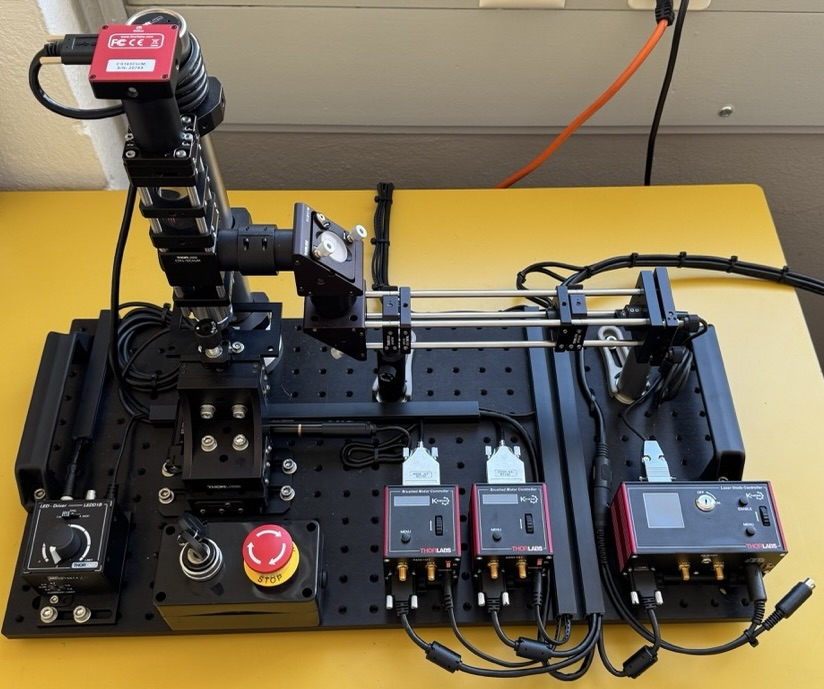
\includegraphics[width=\textwidth]{assets/figures/Cablage_du_kit/Cablage_vierge.jpeg}
    \end{center}
    \caption{Câblage du système sans annotations}
    \label{cablage_kit_pas_annoté}
\end{figure}

\newpage
Une photo du câblage avec des annotations pour une bonne compréhension du travail réalisé est présentée à la Figure \ref{cablage_kit_annoté}.

\begin{figure}[H]
    \centering

    \begin{subfigure}[t]{0.65\textwidth}
        \centering
        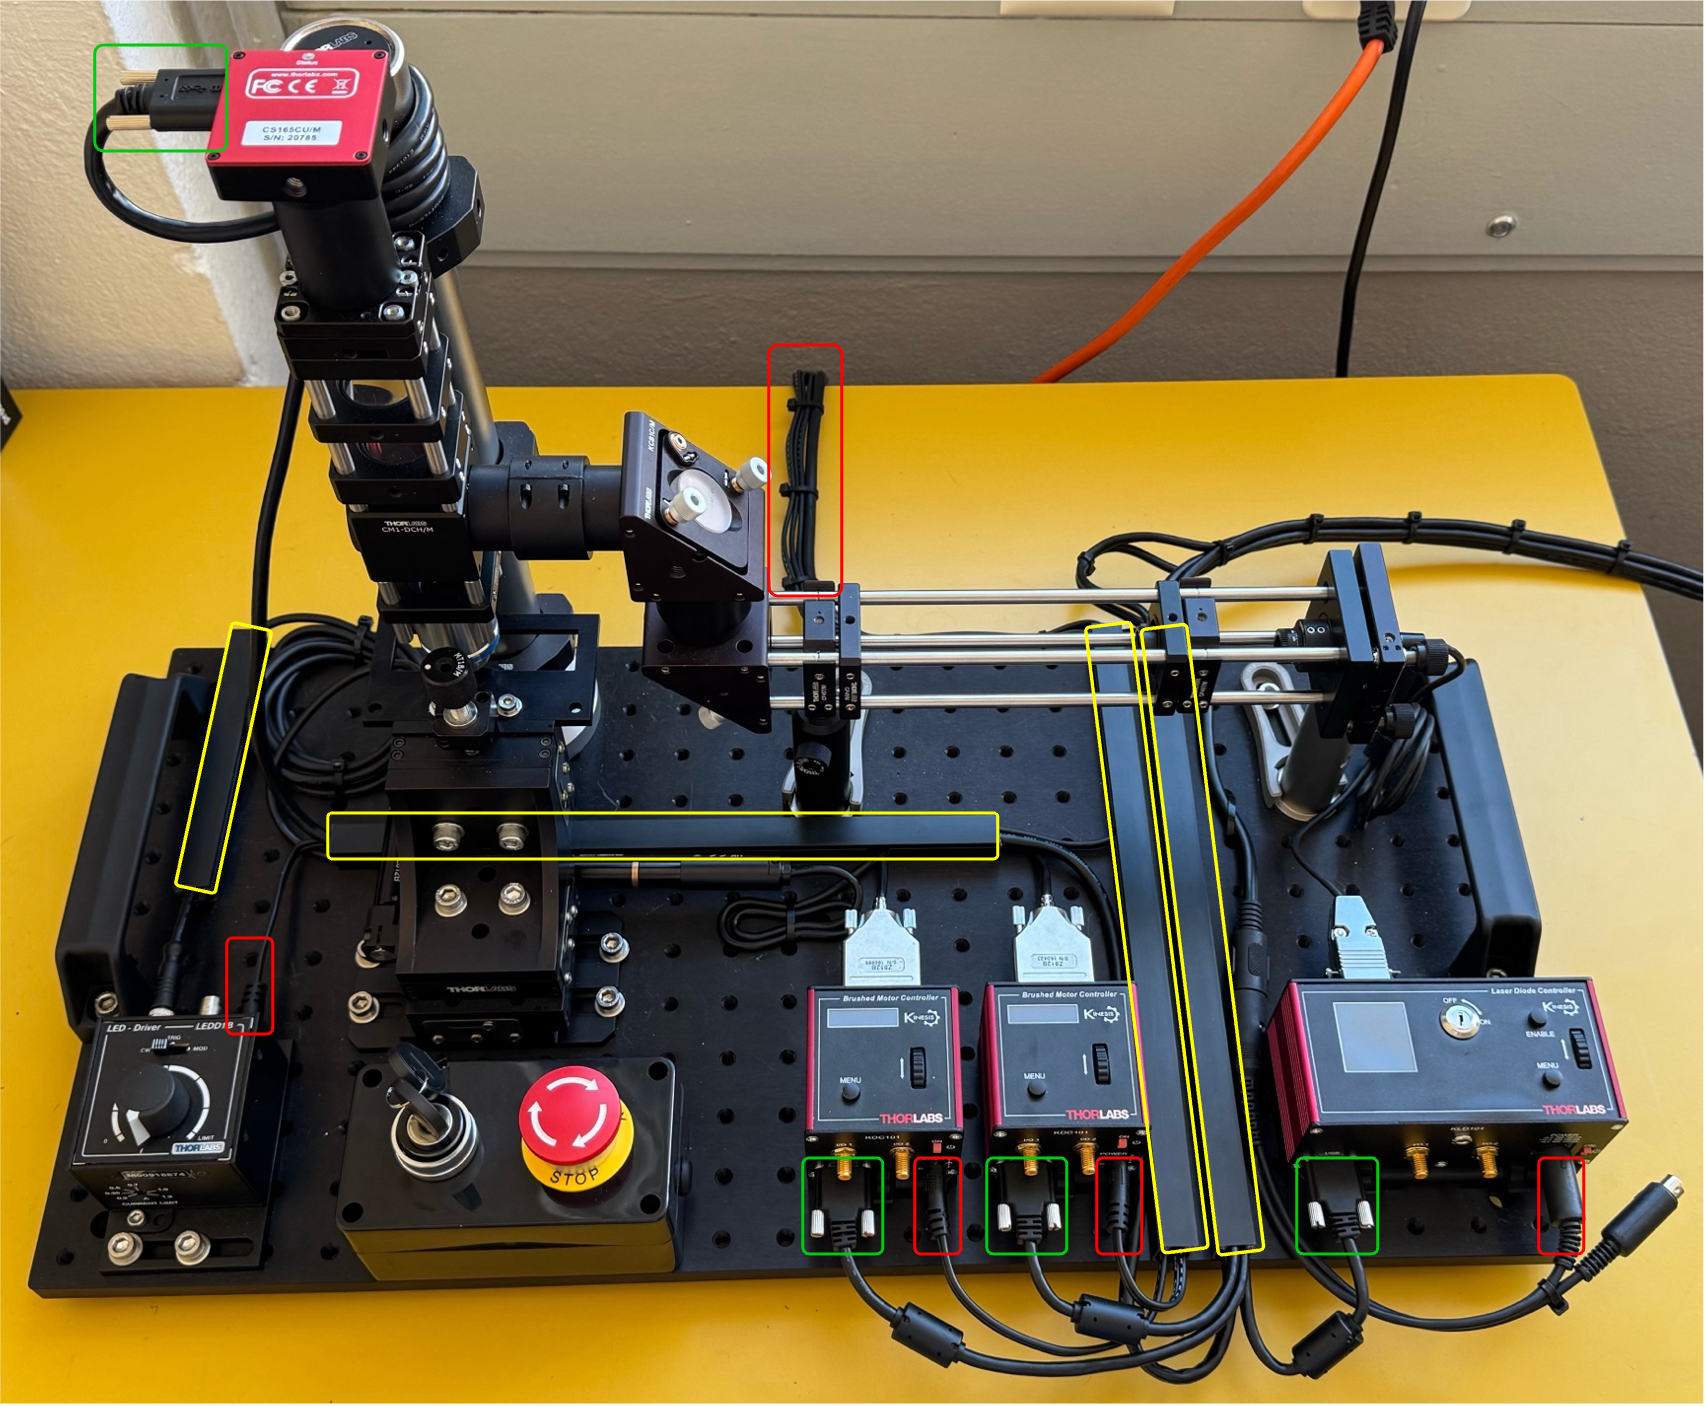
\includegraphics[height=7.5cm]{assets/figures/Cablage_du_kit/cablage_vierge_annote.png}
        \caption{}
        \label{cablage_systeme_complet}
    \end{subfigure}
    \hfill
    \begin{subfigure}[t]{0.25\textwidth}
        \centering
        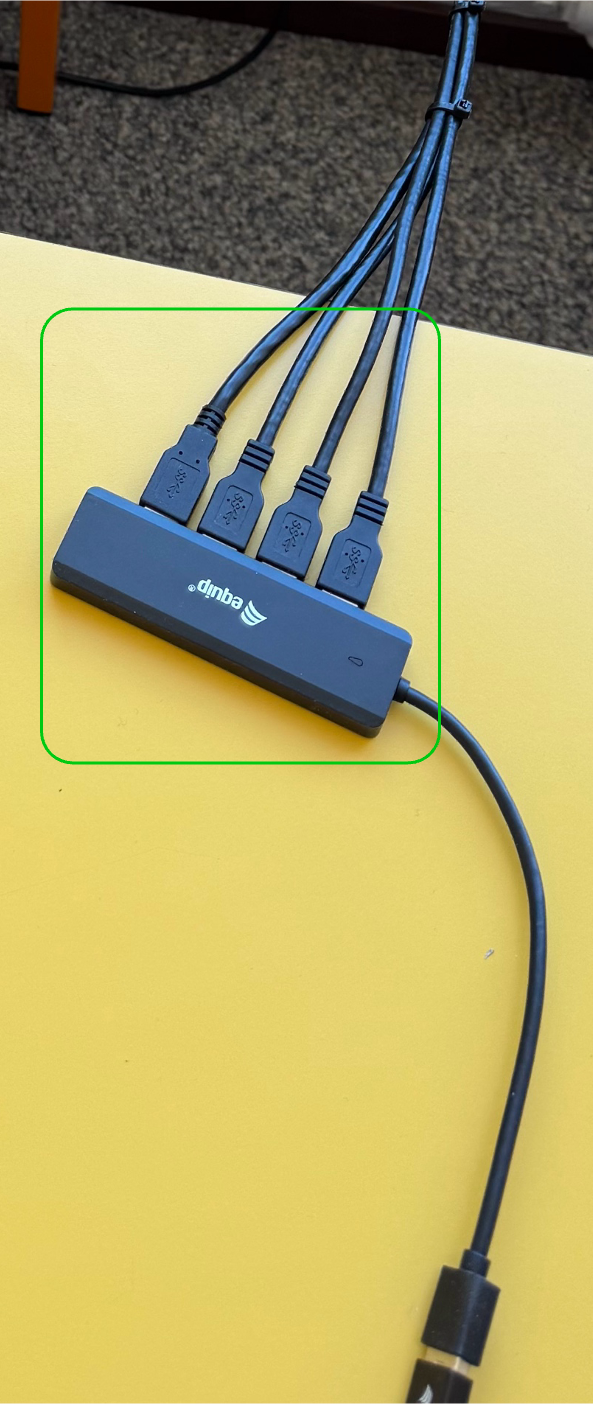
\includegraphics[height=7.5cm]{assets/figures/Cablage_du_kit/Hub_USB_annote.png}
        \caption{}
        \label{cablage_hub_usb}
    \end{subfigure}

    \vskip\baselineskip
    \begin{subfigure}[t]{0.9\textwidth}
        \centering
        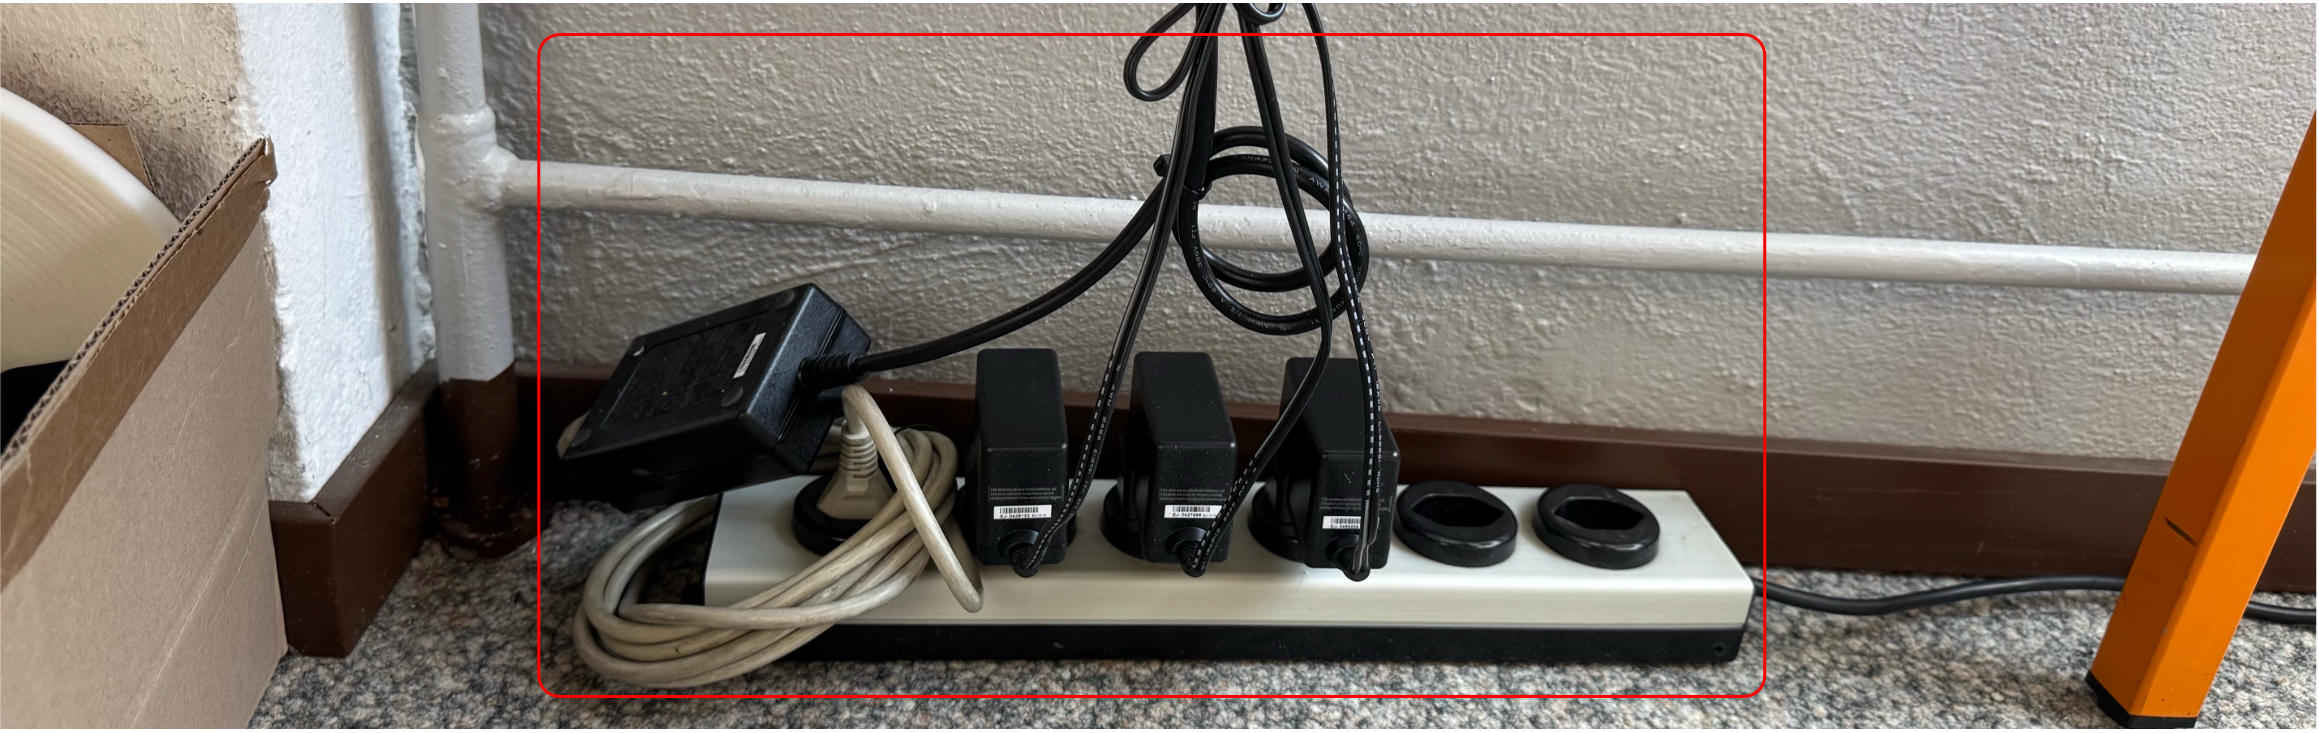
\includegraphics[width=\textwidth]{assets/figures/Cablage_du_kit/Cables_alimentation_annote.png}
        \caption{}
        \label{cablage_alimentation}
    \end{subfigure}

    \caption{Câblage du système avec annotations: a) système complet, b) hub USB-A, c)~alimentations des composants}
    \label{cablage_kit_annoté}
\end{figure}

On peut apercevoir en \textcolor[RGB]{230, 230, 0}{jaune}, que des goulottes ont été installées afin que les câbles tiennent en place, mais également afin d'avoir un visuel au propre.

Les encadrés en \textcolor{red}{rouge} sont les quatre alimentations. Celles-ci sont utilisées pour :
\begin{itemize}[label=\textbullet]
    \item Les deux drivers des servomoteurs
    \item Le driver du laser
    \item Le driver de la LED
\end{itemize}
\vspace{0.5em}
En complément des alimentations, les encadrés en \textcolor[RGB]{0, 201, 18}{vert} désignent les câbles permettant de communiquer avec les différents composants. Voici la liste des câbles pour la communication :
\begin{itemize}[label=\textbullet]
    \item Un câble pour chaque driver de servomoteur, deux au total
    \item Un câble pour le driver du laser
    \item Un câble pour la caméra
\end{itemize}
\vspace{0.5em}
Tous les câbles de communications sont connectés à un hub USB-A, voir la Figure~\ref{cablage_hub_usb}, afin d'avoir en sortie plus qu'un seul câble à brancher au PC.